\documentclass[a4paper,twocolumn]{article}
\usepackage{graphicx}
\usepackage{listings}
\usepackage[justification=centering]{caption}
\usepackage{subfigure}  
\usepackage{multirow}
\lstset{language=Matlab}
\lstset{breaklines}
\lstset{extendedchars=false}

\usepackage{amsmath,amsfonts,amsthm,amssymb}
\theoremstyle{definition}
\newtheorem{thm}{Theorem}
\newtheorem{exmp}{Example}
\newtheorem{defn}{Definition}
\newtheorem{lema}{Lemma}
\newtheorem{prop}{Proposition}
\newtheorem{coro}{Corollary}


\renewcommand{\baselinestretch}{1.25}

%------------setlength----------------%
\setlength{\textwidth}{162mm}
%\setlength{\textheight}{190mm}
\setlength{\textheight}{231mm}
\setlength{\headheight}{-0.1cm}
\setlength{\topmargin}{-0.1cm}
\setlength{\oddsidemargin}{-0cm}
\setlength{\evensidemargin}{-0cm}

\setlength{\parskip}{1mm}
\setlength{\unitlength}{1mm}
\setlength{\parindent}{2em}

\title{Project 1}

\author{Li Zhiqi\quad3180103041}

\begin{document}
\maketitle
\section{Restatement of problem}
The problem to be solved is the restricted three-body system model. In the system, the two heavy bodies are regarded as revolving in fixed orbits about their common centre of mass while the small body is attracted by the heavy bodies but never affecting their motion.\\  We use $u_1,u_2$ and $u_3$ to represent position coordinates of the small body, and use $u_4,u_5$ and $u_6$ to represent the corresponding velocity coordinates. Then the equations of motion are
$$
\left\{\begin{aligned}
u_{1}^{\prime}=& u_{4} \\
u_{2}^{\prime}=& u_{5} \\
u_{3}^{\prime}=& u_{6} \\
u_{4}^{\prime}=& 2 u_{5}+u_{1}-\frac{\mu\left(u_{1}+\mu-1\right)}{\left(u_{2}^{2}+u_{3}^{2}+\left(u_{1}+\mu-1\right)^{2}\right)^{3 / 2}} \\
&-\frac{(1-\mu)\left(u_{1}+\mu\right)^{2}}{\left(u_{2}^{2}+u_{3}^{2}+\left(u_{1}+\mu\right)^{2}\right)^{3 / 2}}, \\
u_{5}^{\prime}=&-2 u_{4}+u_{2}-\frac{\mu u_{2}}{\left(u_{2}^{2}+u_{3}^{2}+\left(u_{1}+\mu-1\right)^{2}\right)^{3 / 2}} \\
&-\frac{(1-\mu) u_{2}}{\left(u_{2}^{2}+u_{3}^{2}+\left(u_{1}+\mu\right)^{2}\right)^{3 / 2}}, \\
u_{6}^{\prime}=&-\frac{\mu u_{3}}{\left(u_{2}^{2}+u_{3}^{2}+\left(u_{1}+\mu-1\right)^{2}\right)^{3 / 2}} \\
&-\frac{(1-\mu) u_{3}}{\left(u_{2}^{2}+u_{3}^{2}+\left(u_{1}+\mu\right)^{2}\right)^{3 / 2}}
\end{aligned}\right.
$$
While the value of $\mu$ = 1/81.45 has been selected. There are two initial values for the problem, and here is Initial1:
$$
\begin{aligned} &\left(u_{1}, u_{2}, u_{3}, u_{4}, u_{5}, u_{6}\right) \\=&(0.994,0,0,0,-2.0015851063790825224,0)
\end{aligned}
$$
and the period is $T_{1}=17.06521656015796 .$\\
Here is Initial2:
$$
\begin{aligned} &\left(u_{1}, u_{2}, u_{3}, u_{4}, u_{5}, u_{6}\right) \\=&(0.87978,0,0,0,-0.3797,0) 
\end{aligned}
$$
and the period if $T_{2}=19.14045706162071 .$\\
For each initial problem, we will use the following methods to solve it:\\\\
\hspace*{1em}\textbf{Adams-Bashforth methods $(p=1,2,3,4)$};\\
\hspace*{1em}\textbf{Adams-Moulton methods $(p=2,3,4,5)$};\\
\hspace*{1em}\textbf{BDFs $(p=1,2,3,4)$};\\
\hspace*{1em}\textbf{the classical Runge-Kutta method}.\\\\
And for each method and initial condition, we're supposed to use a stable time-step to compute the problem to period $T$. Furthermore, by some ways (Periodicity for initial1, and Richardson extrapolation for initial2) we can compute the errors of the problems, and perform a sequence of grid refinement test to analyze the convergence of each method. Finally, we will compare different methods with their total CPU time achieving an error of $10^{-3}$ based on the max-norm of the solution error.
\newpage
\section{Mathematical theory}
\newpage
\section{Calculation results}
In my program, it is necessary to do calculations by writing a input file where the name, order, time-step and other information are given.The specific format is as follows:
\begin{table}[!htp]
	\centering
	\begin{tabular}{|c|c|c|c|}
		\hline	
		Index & Method & Order & dt \\
		\hline		
		1 & BDFs & 3 & 0.0004   \\	
		\hline		
		2 & Runge-Kutta & 0 & 0.0001   \\	
		\hline \hline
		Initial & N & err-analysis & grid-refine-analysis \\
		\hline
		Initial2 & 30000 & 1 & 1 \\
		\hline
		Initial1 & 200000 & 1 & 0 \\
		\hline
	\end{tabular}
	\caption{Input format}
	\label{tab:format}
\end{table}\\
In the above input format, err-analysis equals to 1 means the solution error will be calculated, otherwise it will only calculate the result; Grid-refine-analysis equals to 1 means the program will perform a sequence of grid refinement test to analyze the convergence of the method.By the way, for order of Runge-Kutta method, you must fill in 0 though it will never be used; If you choose Initial1 as initial condition and calculate the error in program, N will not be used for we calculate the solution error by periodicity.\\
You can use the command \textbf{"make run"} to get some test results. Exit matlab to get the next picture.

%1.two plots of solution make test1
\subsection{Two example plots of solution}
Firstly, we take Euler's method and classical Runge-Kutta as examples to show the general effect of results. The input file is as follows:\\
\begin{table}[!htp]
	\centering
	\begin{tabular}{|c|c|c|c|}
		\hline	
		Index & Method & Order & dt \\
		\hline		
		1 & Adams-Bashforth & 1 & 0.000711   \\	
		\hline		
		2 & Runge-Kutta & 0 & 0.002844   \\	
		\hline \hline
		Initial & N & err & grid-refine \\
		\hline
		Initial1 & 24000 & 0 & 0 \\
		\hline
		Initial1 & 6000 & 0 & 0 \\
		\hline
	\end{tabular}
	\caption{Input test1}
	\label{tab:test1}
\end{table}\\
You can use the command \textbf{"make test1"} to get the result.Exit matlab to get the next picture.\\
Here are outputs and plots from the program:\\\\
\emph{Problem 1: relust: (1.3888,1.89075,0),}\\
\emph{CPU time: 76.468(ms)}\\
\emph{Problem 2: relust: (0.761211,-0.259659,0),}\\
\emph{CPU time: 67.922(ms)}\\
\begin{figure}[!htp]   
	\centering
	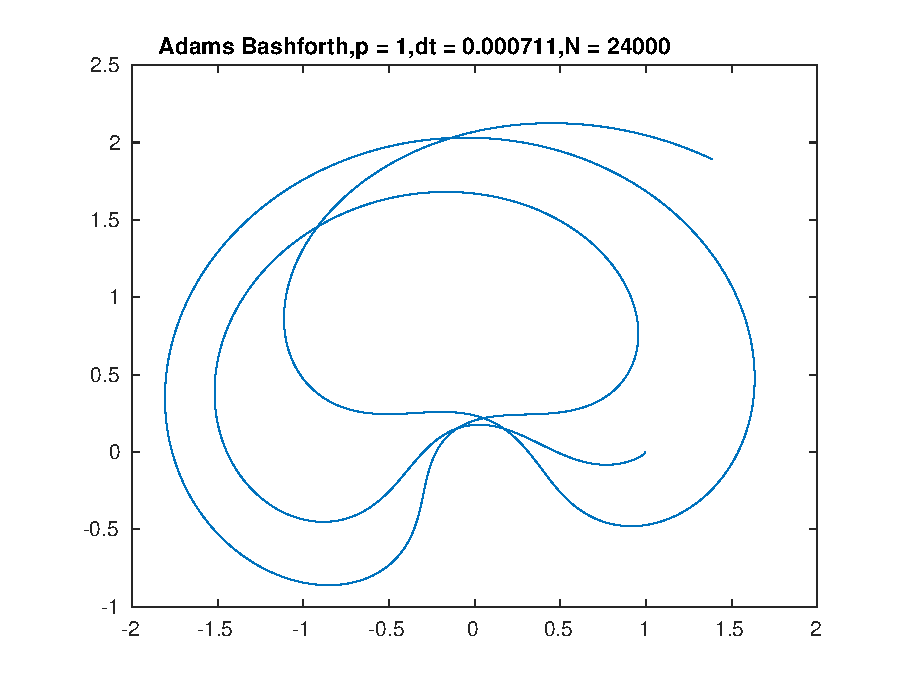
\includegraphics[width=8cm]{Pictures/1_1.eps}
	\caption{Euler's Method, 24000 steps}
	\label{fig:Euler24000}
\end{figure}
\begin{figure}[!htp]   
	\centering
	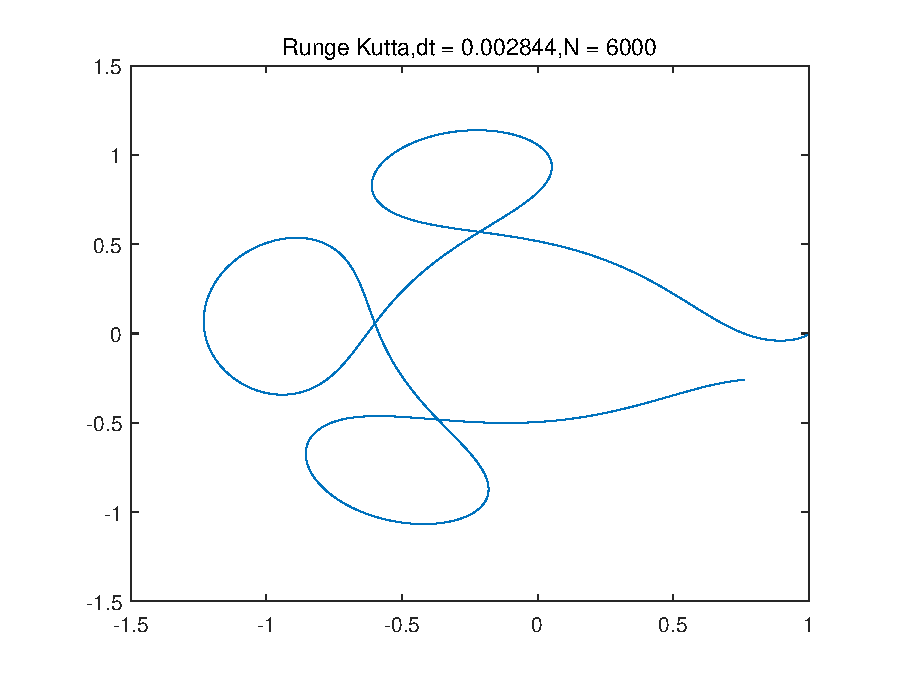
\includegraphics[width=8cm]{Pictures/1_2.eps}
	\caption{classical Runge-Kutta Method, 6000 steps}
	\label{fig:RK6000}
\end{figure}\\
Obviously 24000 steps Euler's Method is not satisfactory for Initial1, while 6000 steps classical Runge-Kutta method performs better but is still inaccurate.
\newpage
%2.有效性分析 2.1 2.2 ... make test2
\subsection{Effectiveness analysis}
In the second part, we will compute the solution error and perform a sequence of grid refinement test to analyze the convergence of each method. We will get the order of convergence which is the criterion of whether the method is effective or not.\\
Use the command \textbf{"make test2"} to get all the result\textbf{(will take much time)}.
\subsubsection{Adams-Bashforth methods analysis}
$p = 1,3$, we take Initial2 as initial condition.\\
$p = 2,4$, we take Initial1 as initial condition.\\
In fact, there is no significant difference between two initial conditions when talking about the order of convergence. So for each $p$, we only show the result of Initial1 or Initial2. The input file is as follows:
\begin{table}[!htp]
	\centering
	\begin{tabular}{|c|c|c|c|}
		\hline	
		Index & Method & Order & dt \\
		\hline		
		1 & Adams-Bashforth & 1 & 0.0004   \\	
		\hline		
		2 & Adams-Bashforth & 2 & 0.0001   \\
		\hline		
		3 & Adams-Bashforth & 3 & 0.0004   \\	
		\hline		
		4 & Adams-Bashforth & 4 & 0.0003   \\	
		\hline \hline
		Initial & N & err & grid-refine \\
		\hline
		Initial2 & 30000 & 0 & 1 \\
		\hline
		Initial1 & 0 & 0 & 1 \\
		\hline
		Initial2 & 30000 & 0 & 1 \\
		\hline
		Initial1 & 0 & 0 & 1 \\
		\hline
	\end{tabular}
	\caption{Input test2-1}
	\label{tab:test21}
\end{table}\\
You can use the command \textbf{"make test21"} to get the result. Here are outputs and plots from the program:\\\\
\emph{Problem 1:Order=1.01572}\\
\emph{Error constant = 2.23187e+03}\\
\emph{Problem 2: Order = 1.92056}\\
\emph{Error constant = 1.55428e+06}\\
\emph{Problem 3: Order = 2.96347}\\
\emph{Error constant = 8.61791e+04}\\
\emph{Problem 4: Order = 4.00685}\\
\emph{Error constant = 1.66229e+12}

\begin{figure}[!htp]   
	\centering
	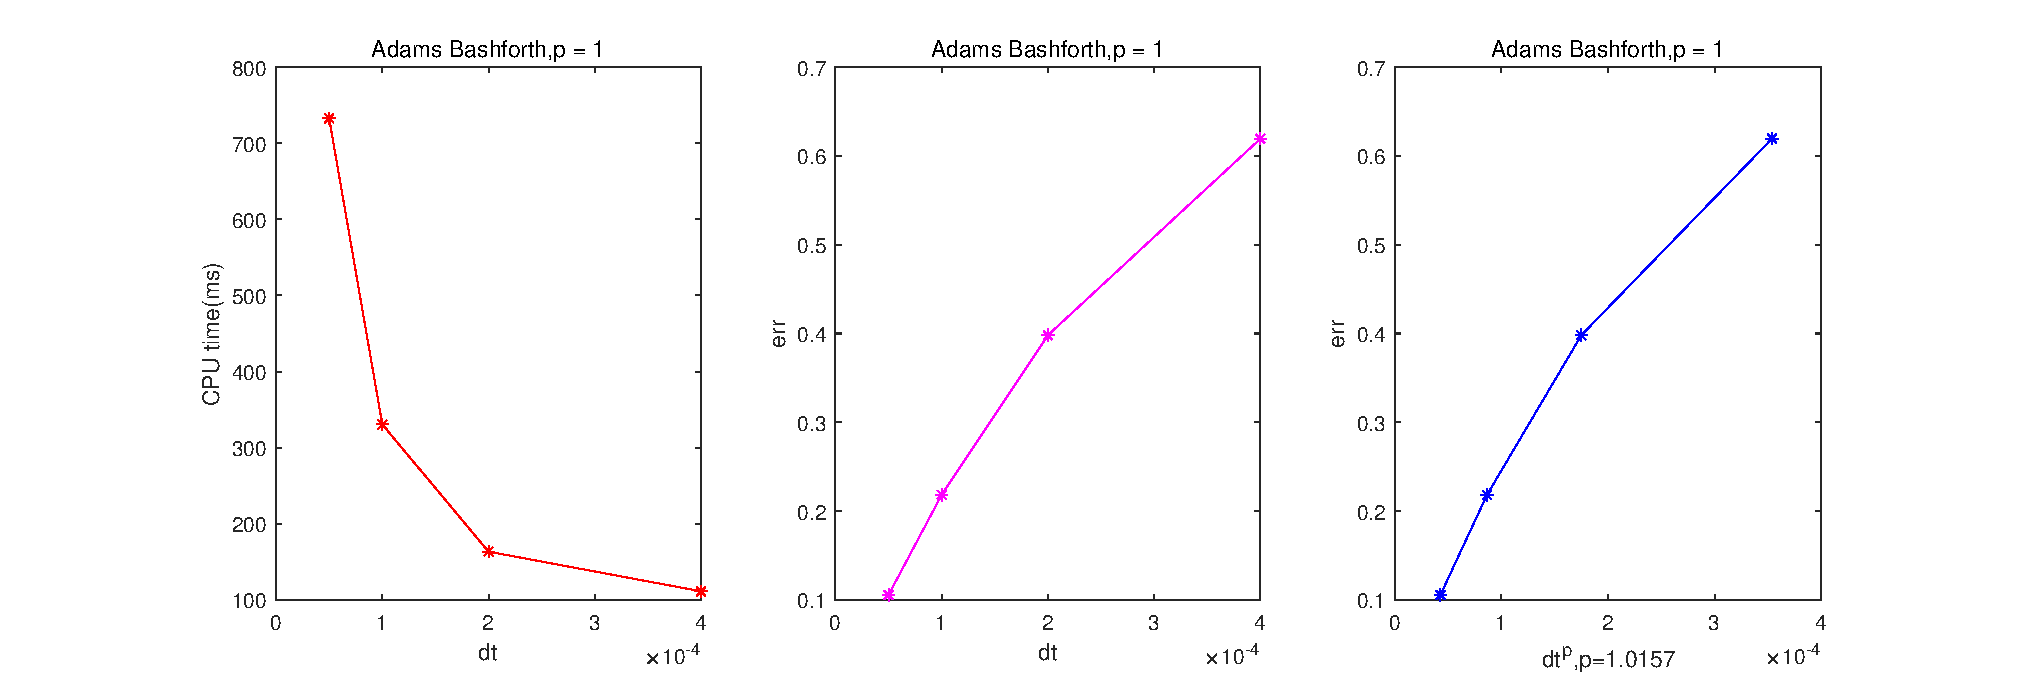
\includegraphics[width=14.2cm]{Pictures/2_1_1.eps}
	\caption{Adams-Bashforth,p=1}
	\label{fig:AB1gf}
\end{figure}
\begin{figure}[!htp]   
	\centering
	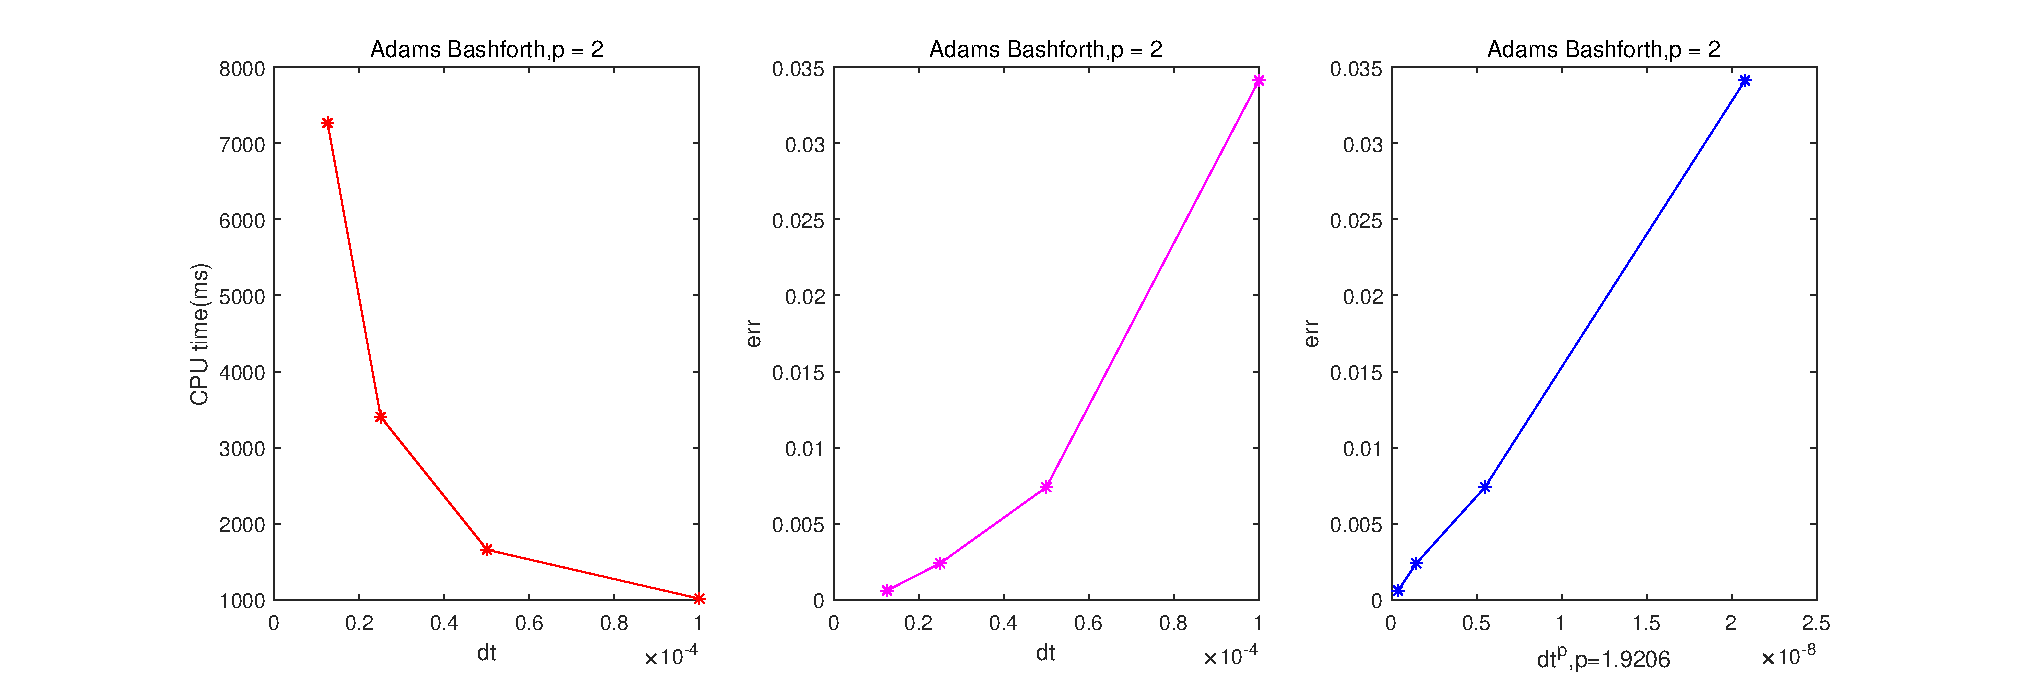
\includegraphics[width=14.2cm]{Pictures/2_1_2.eps}
	\caption{Adams-Bashforth,p=2}
	\label{fig:AB2gf}
\end{figure}
\begin{figure}[!htp]   
	\centering
	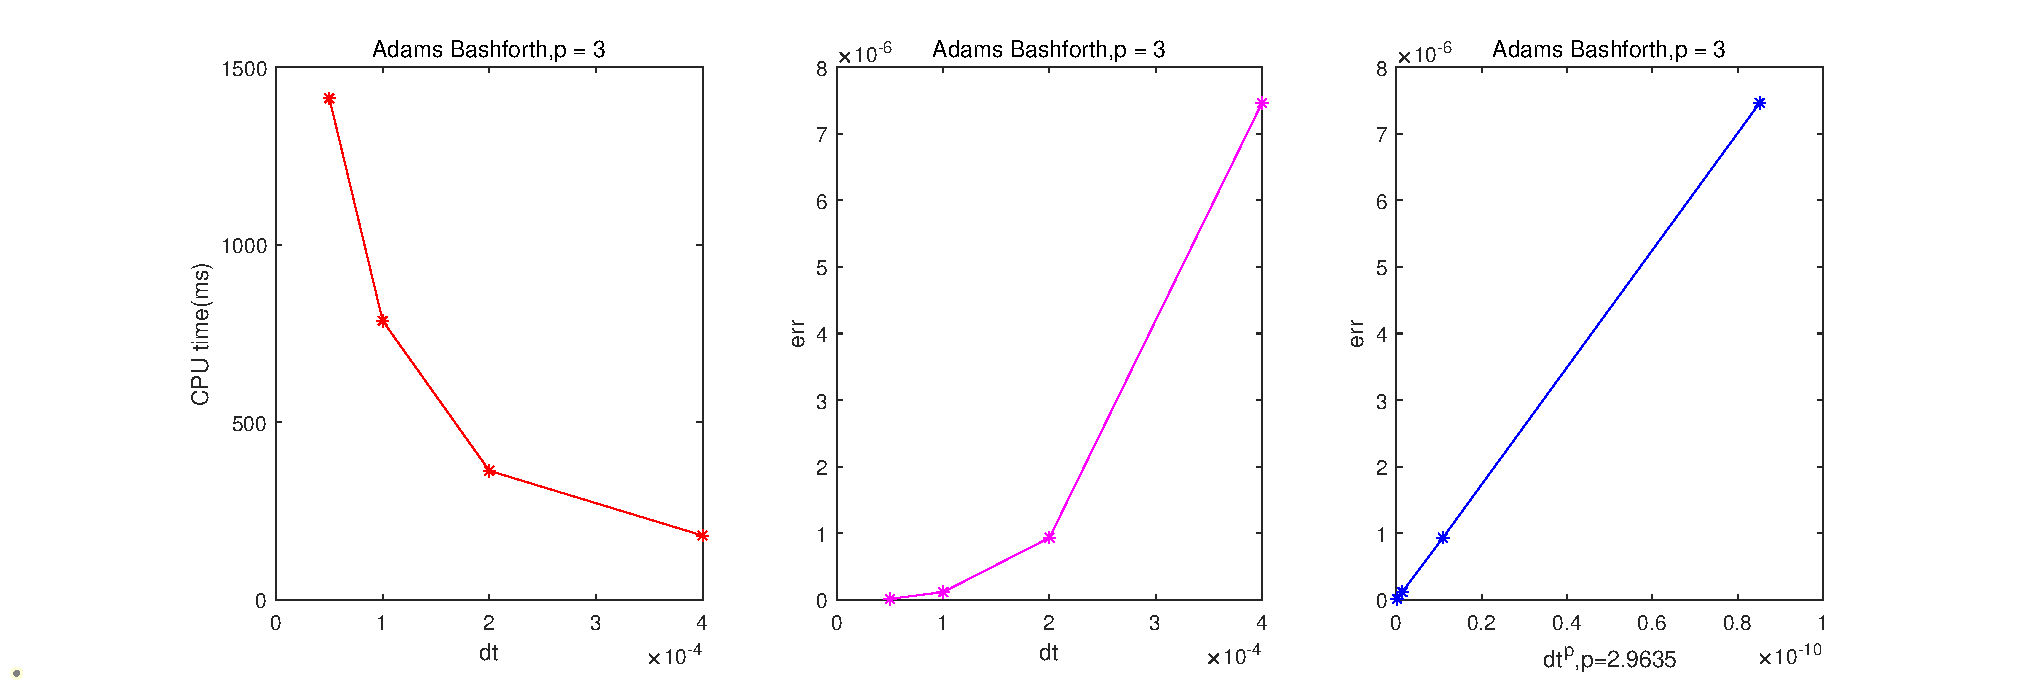
\includegraphics[width=14.2cm]{Pictures/2_1_3.eps}
	\caption{Adams-Bashforth,p=3}
	\label{fig:AB3gf}
\end{figure}
\begin{figure}[!htp]   
	\centering
	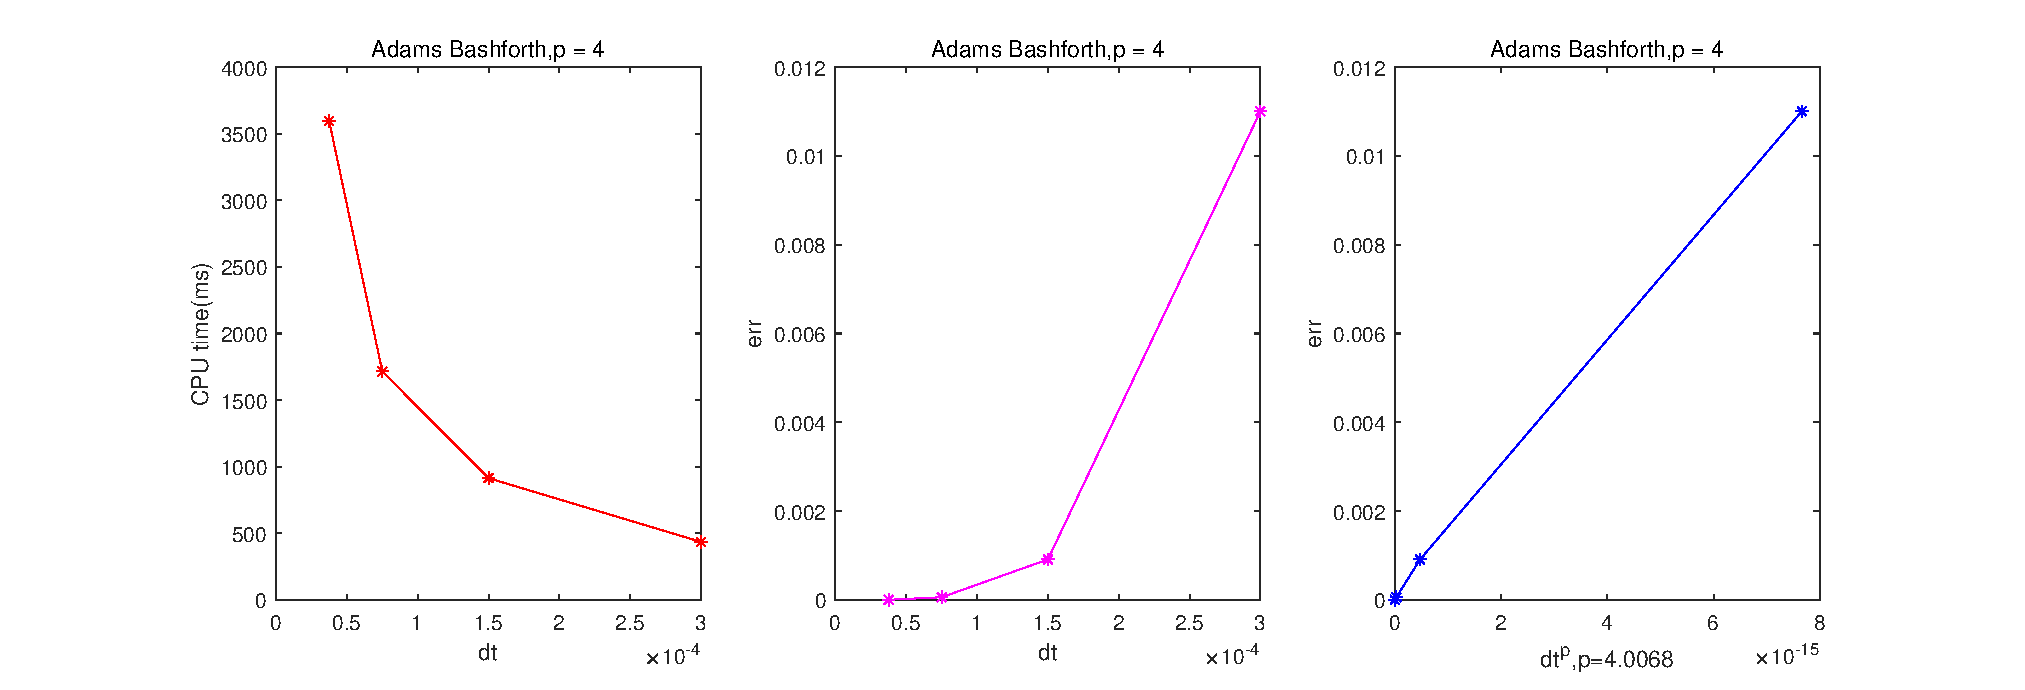
\includegraphics[width=14.2cm]{Pictures/2_1_4.eps}
	\caption{Adams-Bashforth,p=4}
	\label{fig:AB4gf}
\end{figure}
\clearpage
\noindent From above results, each method fits its order of convergence well, so we draw a conclusion that the program of Adams-Bashforth method is effective. 
\subsubsection{Adams-Moulton methods analysis}
As space is limited and to avoid meaningless repetition, we only consider cases $p$=3 and $p$=5, using Initial2 and Initial1  respectively. Other cases are similar. Here is input file:
\begin{table}[!htp]
	\centering
	\begin{tabular}{|c|c|c|c|}
		\hline	
		Index & Method & Order & dt \\
		\hline		
		1 & Adams-Moulton & 3 & 0.0004   \\	
		\hline		
		2 & Adams-Moulton & 5 & 0.0004   \\	
		\hline \hline
		Initial & N & err & grid-refine \\
		\hline
		Initial2 & 30000 & 0 & 1 \\
		\hline
		Initial1 & 0 & 0 & 1 \\
		\hline
	\end{tabular}
	\caption{Input test2-2}
	\label{tab:test22}
\end{table}\\
Use the command \textbf{"make test22"} to get the result. Here are outputs and plots from the program:\\\\
\emph{Problem 1:Order=2.72619}\\
\emph{Error constant = 1.34139e+03}\\
\emph{Problem 2: Order = 4.35899}\\
\emph{Error constant = 2.0824e+11}

\begin{figure}[!htp]   
	\centering
	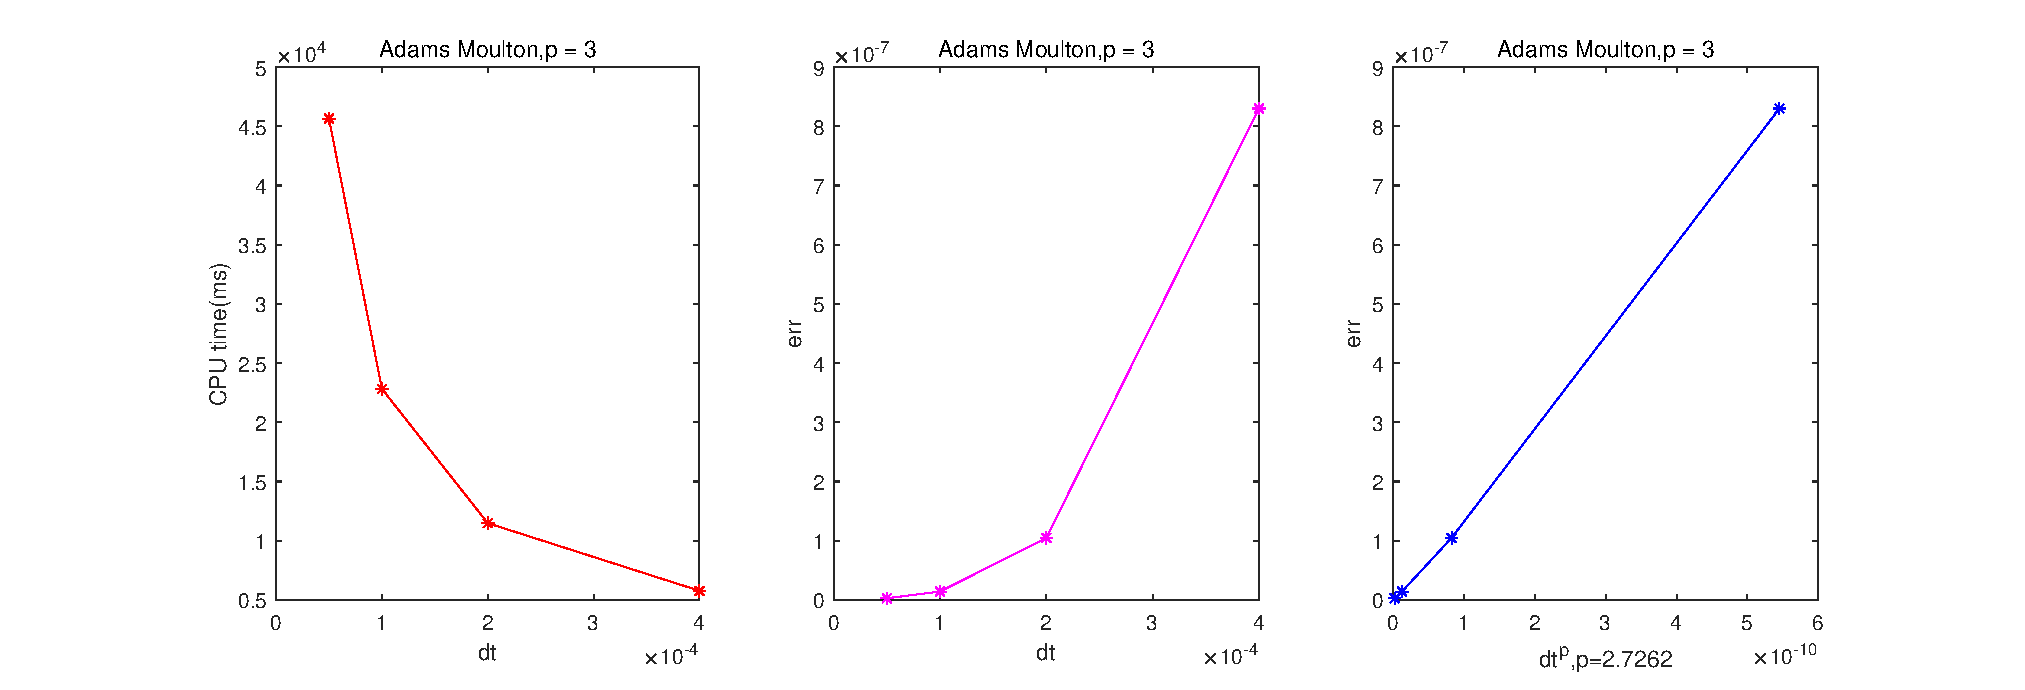
\includegraphics[width=9cm]{Pictures/2_2_1.eps}
	\caption{Adams-Moulton,p=3}
	\label{fig:AM3gf}
\end{figure}
\begin{figure}[!htp]   
	\centering
	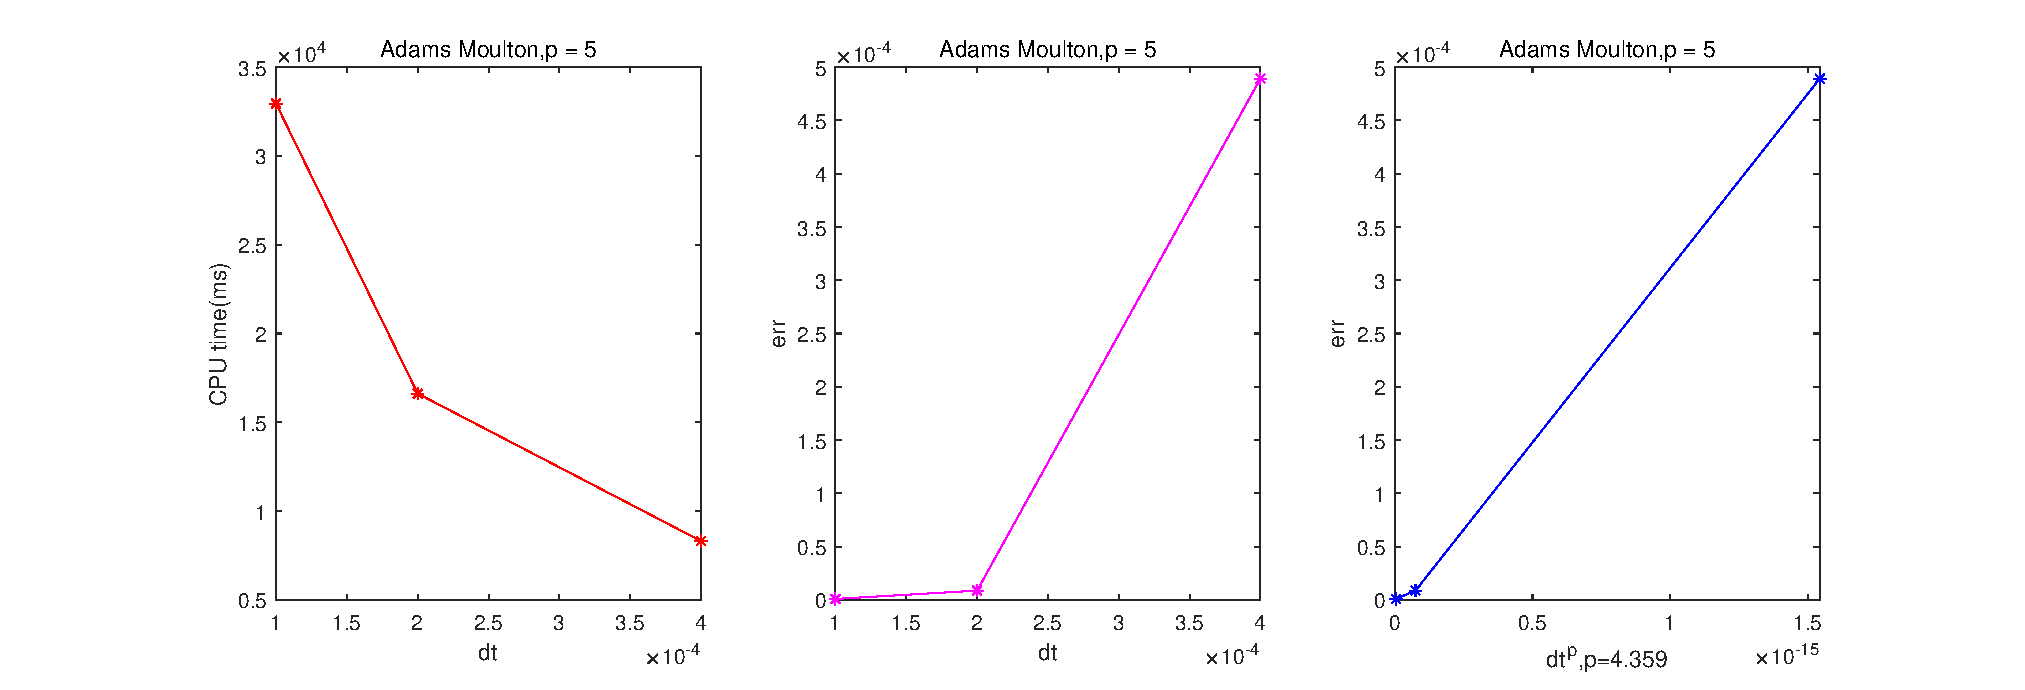
\includegraphics[width=9cm]{Pictures/2_2_2.eps}
	\caption{Adams-Moulton,p=5}
	\label{fig:AM5gf}
\end{figure}
\noindent We can find that Adams-Moulton methods have worse performance compared with Adams-Bashforth methods resulting from round-off error. But in general the order of convergence is close to the theoretical value, so we also draw the conclusion that the program of Adams-Moulton method is effective. 
\subsubsection{BDF methods analysis}
For the same reason as Adams-Moulton mathods, we only consider cases $p$=1 and $p$=3, using Initial1 and Initial2  respectively. Here is input file:
\begin{table}[!htp]
	\centering
	\begin{tabular}{|c|c|c|c|}
		\hline	
		Index & Method & Order & dt \\
		\hline		
		1 & BDFs & 1 & 0.0001   \\	
		\hline		
		2 & BDFs & 3 & 0.0004   \\	
		\hline \hline
		Initial & N & err & grid-refine \\
		\hline
		Initial1 & 0 & 0 & 1 \\
		\hline
		Initial2 & 20000 & 0 & 1 \\
		\hline
	\end{tabular}
	\caption{Input test2-3}
	\label{tab:test23}
\end{table}\\
Use the command \textbf{"make test23"} to get the result. Here are outputs and plots from the program:\\\\
\emph{Problem 1:Order=1.04632}\\
\emph{Error constant = 6084.69}\\
\emph{Problem 2: Order = 2.73333}\\
\emph{Error constant = 722.068}\\\\\\\\
\begin{figure}[!htp]   
	\centering
	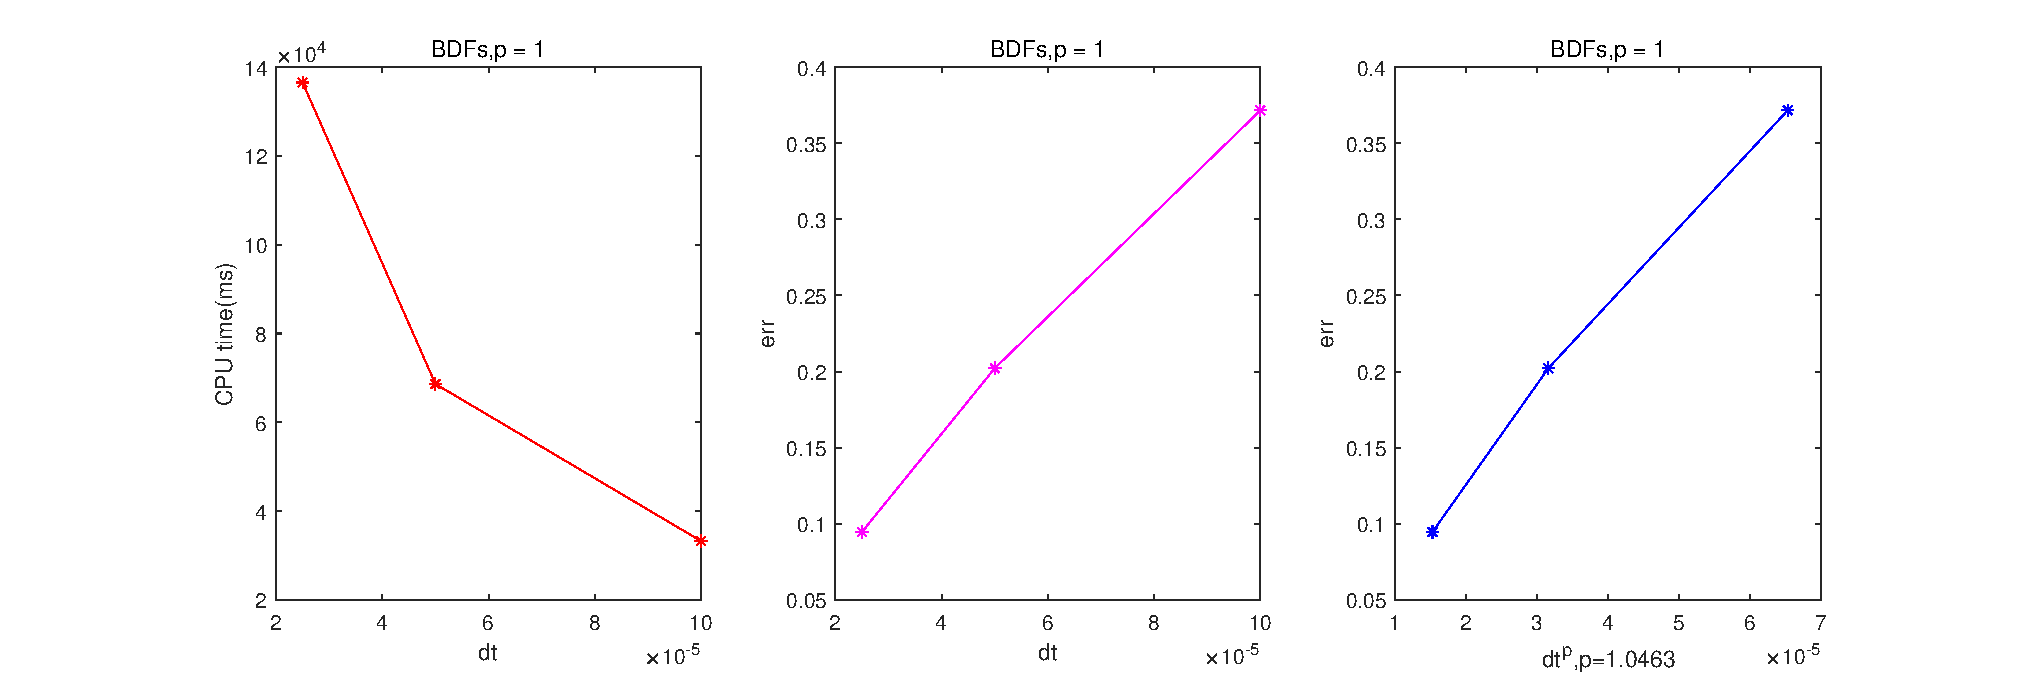
\includegraphics[width=9cm]{Pictures/2_3_1.eps}
	\caption{BDF,p=1}
	\label{fig:BDF1gf}
\end{figure}
\newpage
\begin{figure}[!htp]   
	\centering
	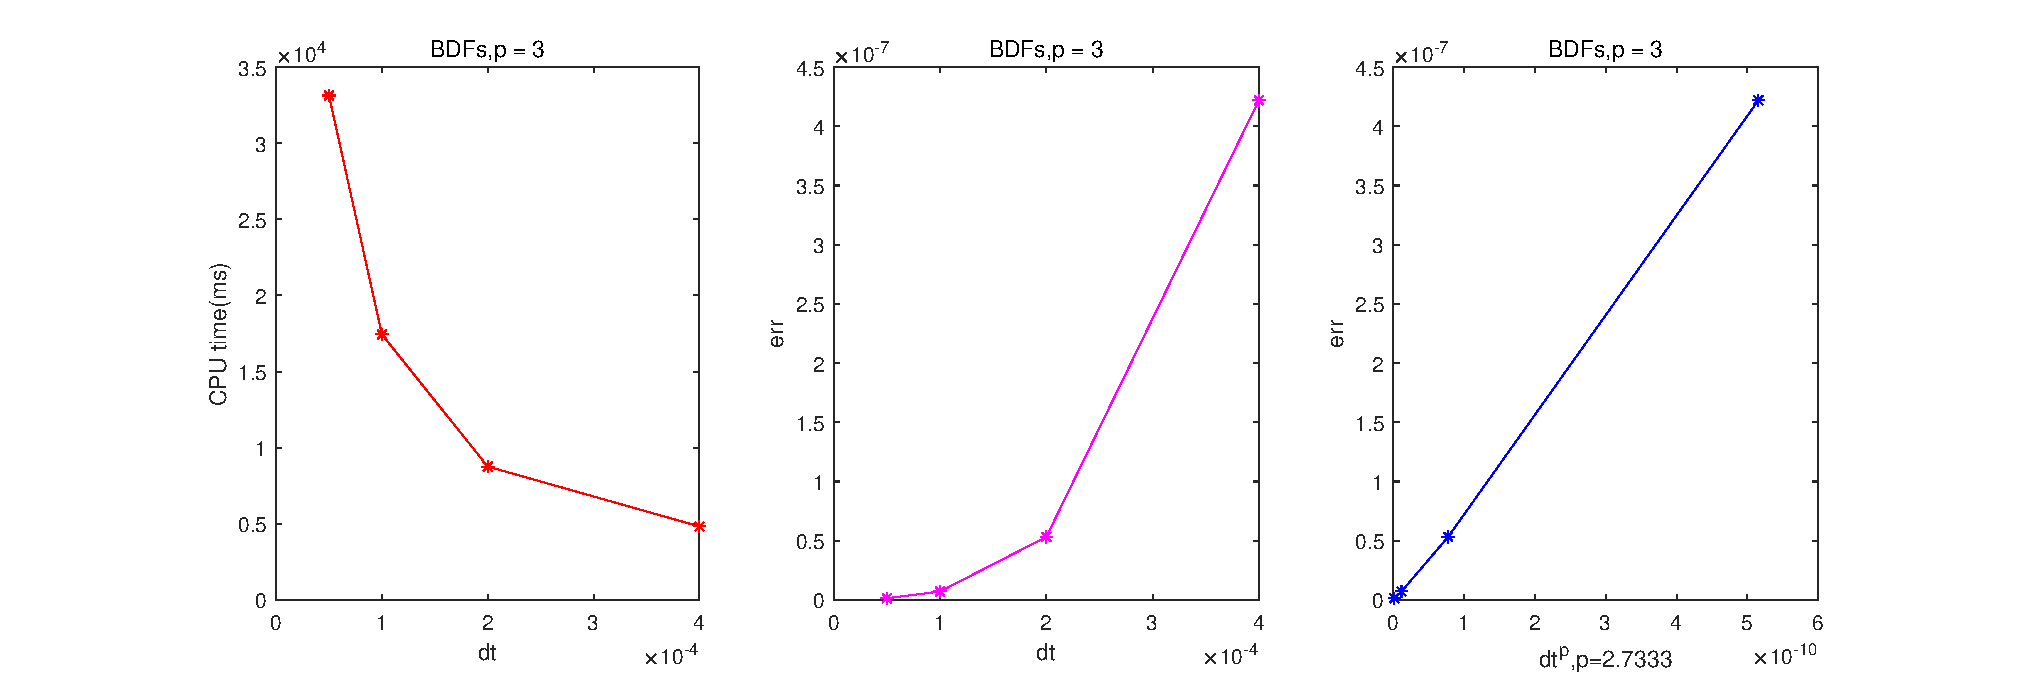
\includegraphics[width=9cm]{Pictures/2_3_2.eps}
	\caption{BDF,p=3}
	\label{fig:BDF3gf}
\end{figure}
\noindent Similar to Adams-Moulton methods, We come to the conclusion that the program of BDFs is effective. 
\subsubsection{Classical Runge-Kutta method analysis}
Classical Runge-Kutta method is convergent with order of
accuracy four. Next we will verify this for Initial1 and Initial2 respectively. The input file is as follows:
\begin{table}[!htp]
	\centering
	\begin{tabular}{|c|c|c|c|}
		\hline	
		Index & Method & Order & dt \\
		\hline		
		1 & Runge-Kutta & 0 & 0.003   \\	
		\hline		
		2 & Runge-Kutta & 0 & 0.005   \\	
		\hline \hline
		Initial & N & err & grid-refine \\
		\hline
		Initial1 & 0 & 0 & 1 \\
		\hline
		Initial2 & 5000 & 0 & 1 \\
		\hline
	\end{tabular}
	\caption{Input test2-4}
	\label{tab:test24}
\end{table}\\
Use the command \textbf{"make test24"} to get the result. Here are outputs and plots from the program:\\\\
\emph{Problem 1:Order=3.97622}\\
\emph{Error constant = 3.52753e+09}\\
\emph{Problem 2: Order = 3.92435}\\
\emph{Error constant = 7.57268e+03}
\begin{figure}[!htp]   
	\centering
	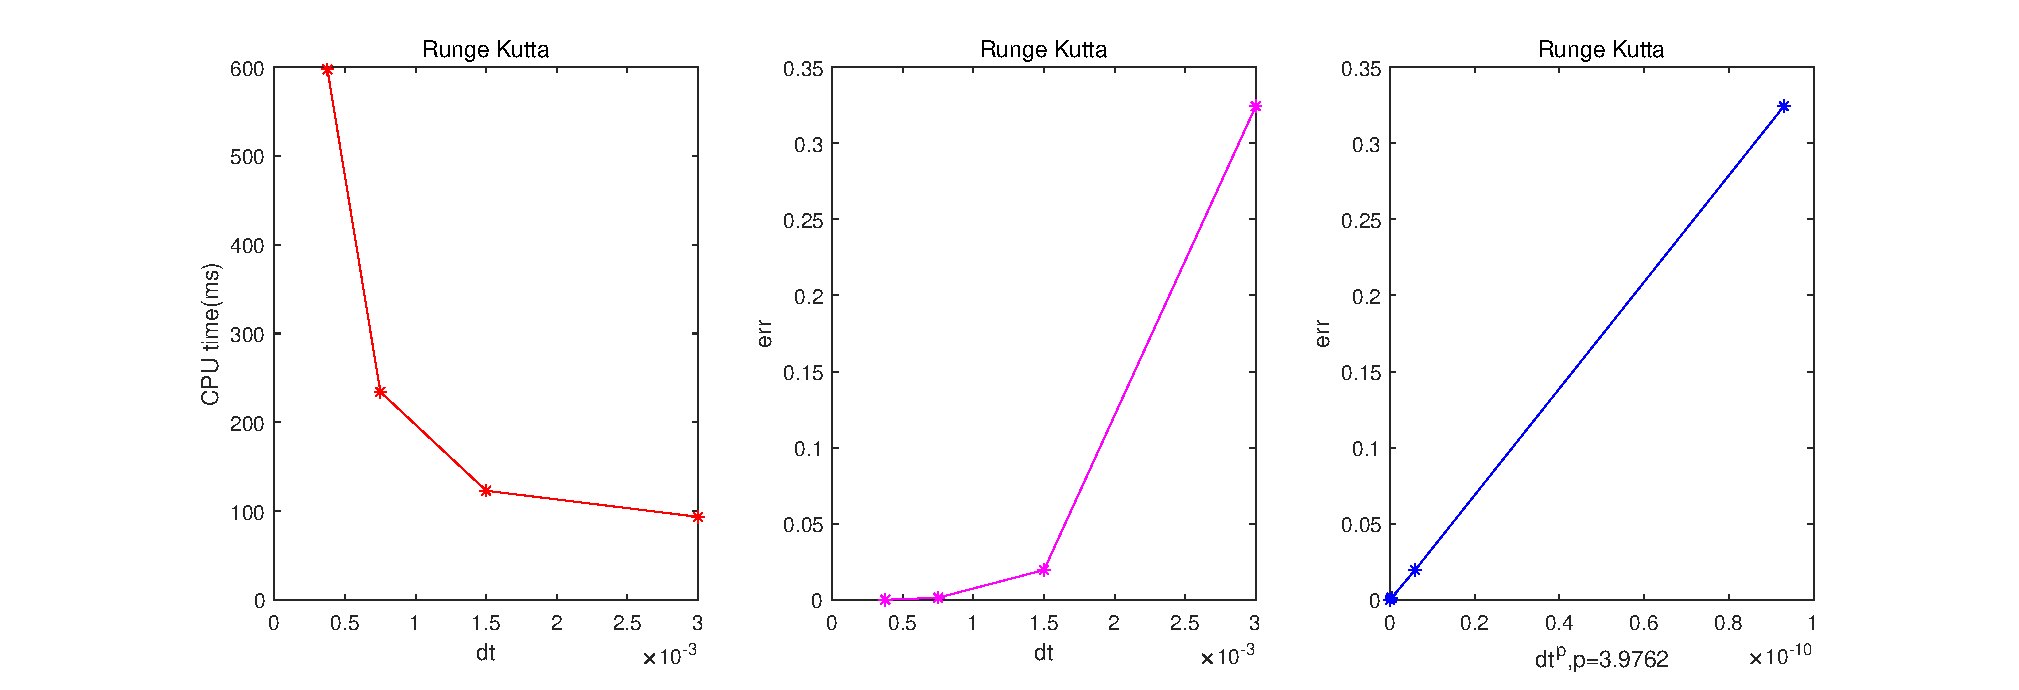
\includegraphics[width=9cm]{Pictures/2_4_1.eps}
	\caption{Runge-Kutta,Initial1}
	\label{fig:RK1gf}
\end{figure}
\newpage
\begin{figure}[!htp]   
	\centering
	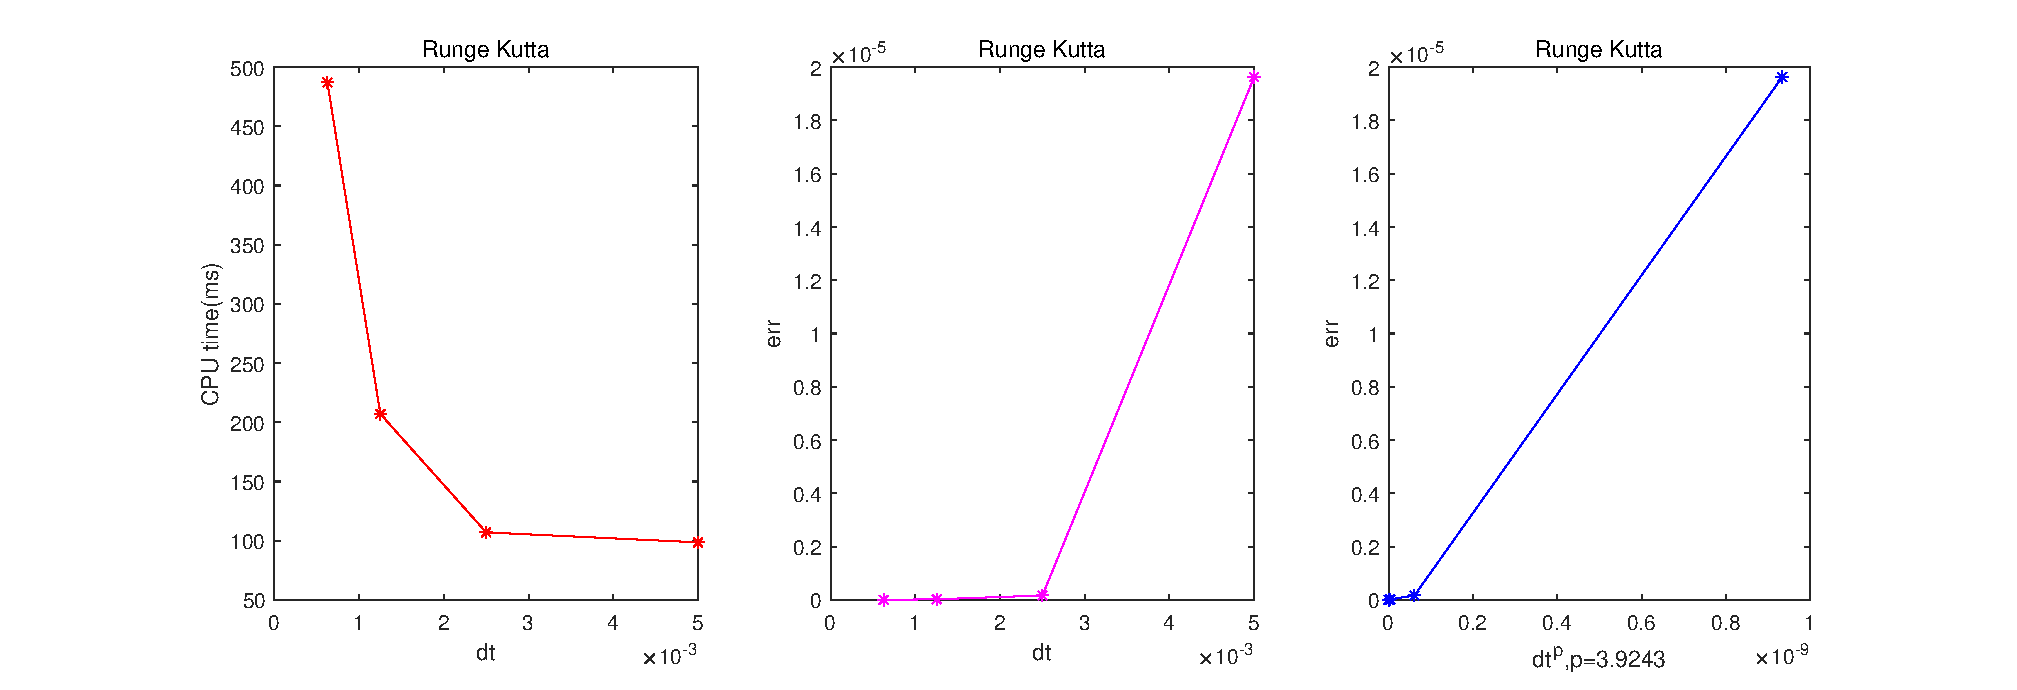
\includegraphics[width=9cm]{Pictures/2_4_2.eps}
	\caption{Runge-Kutta,Initial2}
	\label{fig:RK2gf}
\end{figure}
\noindent There's no doubt that classical Runge-Kutta method performs much well and it's effective.
%3.关键步长 每种方法取一个p make test3
\subsection{Determination of key time-step size}
In this part, We will report a time-step size with which the plot of the solutions is visually indistinguishable from the corresponding plot given by problem. Because the property of the problem is different under the two different initial value conditions, we will discuss them separately.
\subsubsection{Time-step size for Initial1}
As reference, the plot of solution for Initial1 is as follows:\\
\begin{figure}[!htp]   
	\centering
	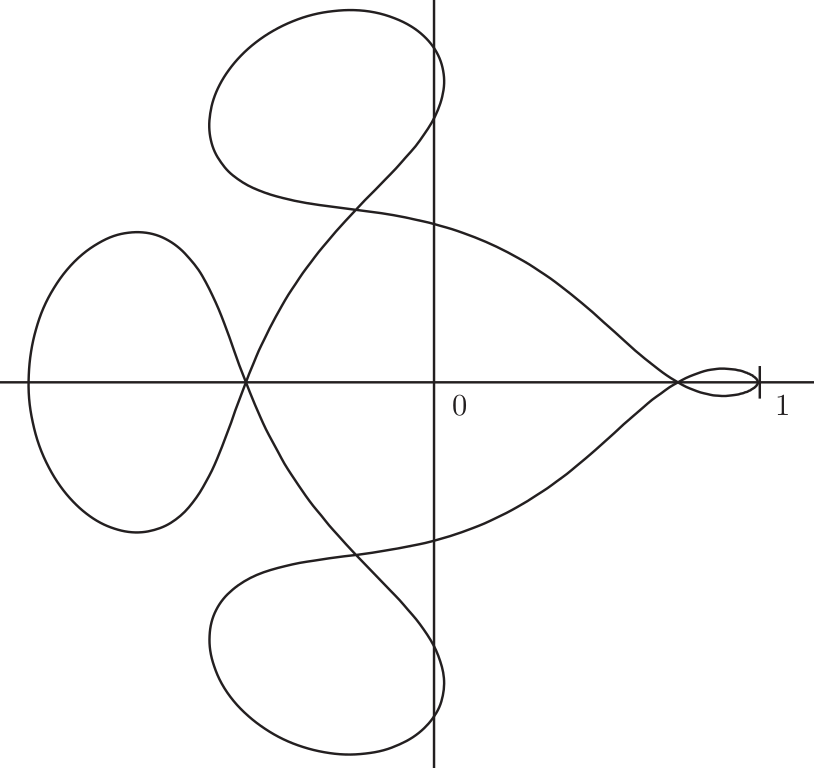
\includegraphics[width=6cm]{Pictures/I1.png}
	\caption{Reference plot for Initial1}
	\label{fig:R1}
\end{figure}\\
\noindent The following is the determination of the key time-step size of each method. You can use the command \textbf{"make test31"} to get all the .m file, and run them to get following plots.
\newpage
\begin{figure}[!htp] 
	\centering
	\subfigure[p = 1, dt = 1e-05]{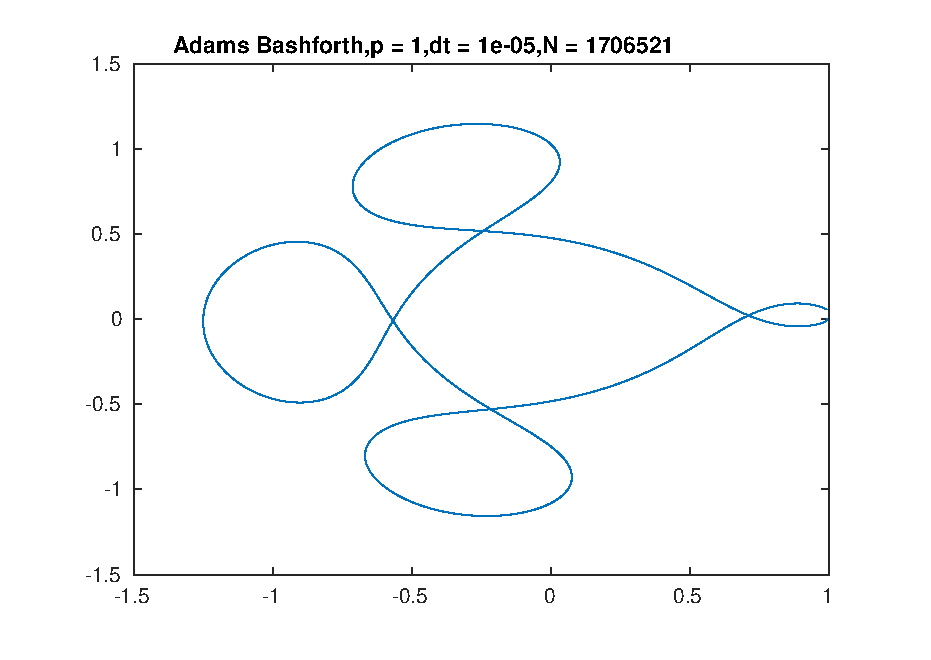
\includegraphics[width=1.5in]{Pictures/3_11.eps}}
	\subfigure[p = 2, dt = 1e-04]{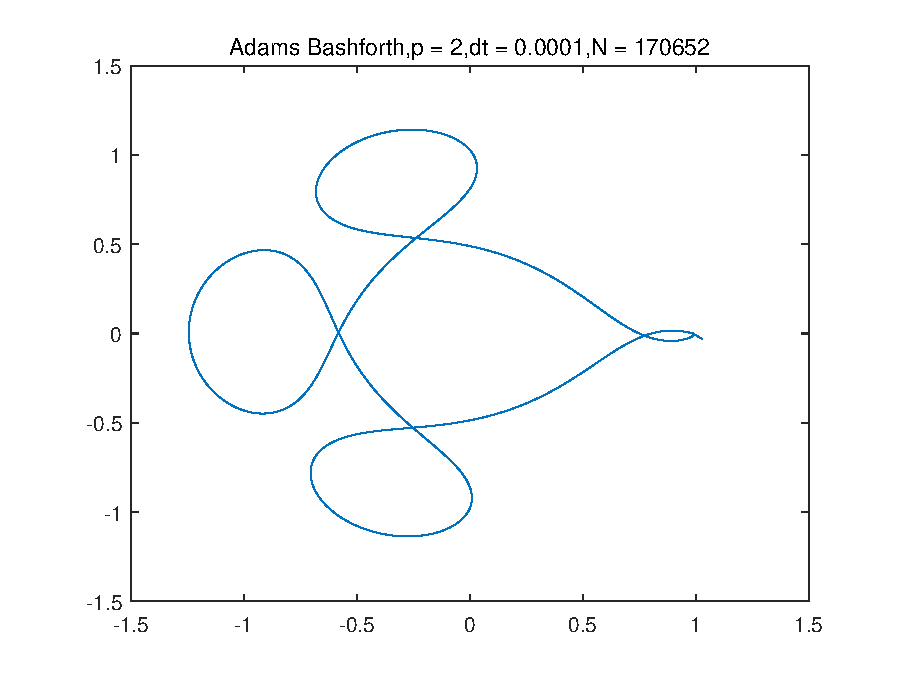
\includegraphics[width=1.5in]{Pictures/3_12.eps}}
	\caption{Adams-Bashforth,p = 1,2 }
	\label{AB1ks}
\end{figure}
\begin{figure}[!htp] 
	\centering
	\subfigure[p = 3, dt = 4e-04]{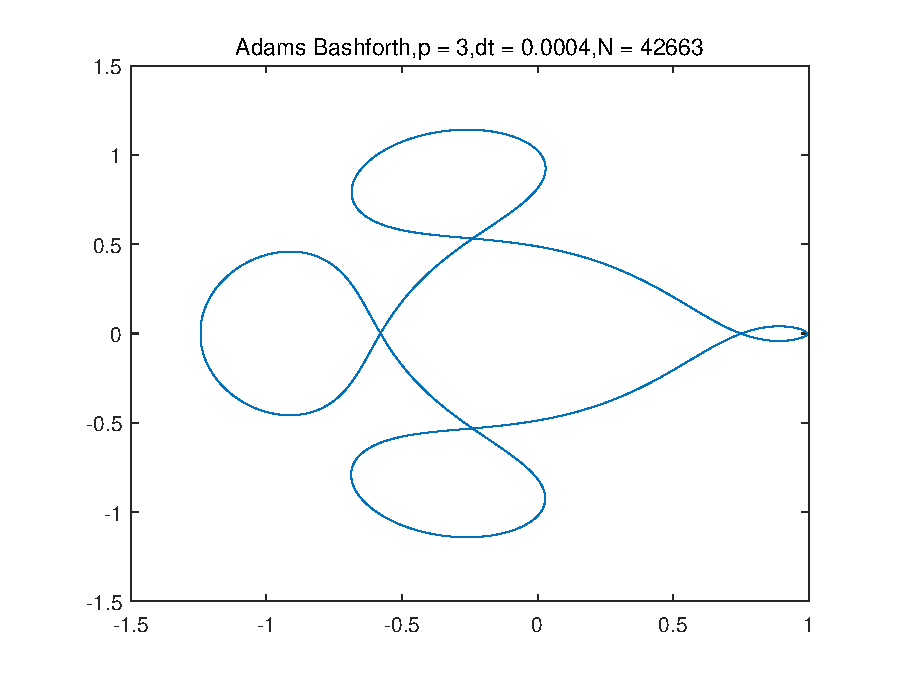
\includegraphics[width=1.5in]{Pictures/3_13.eps}}
	\subfigure[p = 4, dt = 8e-05]{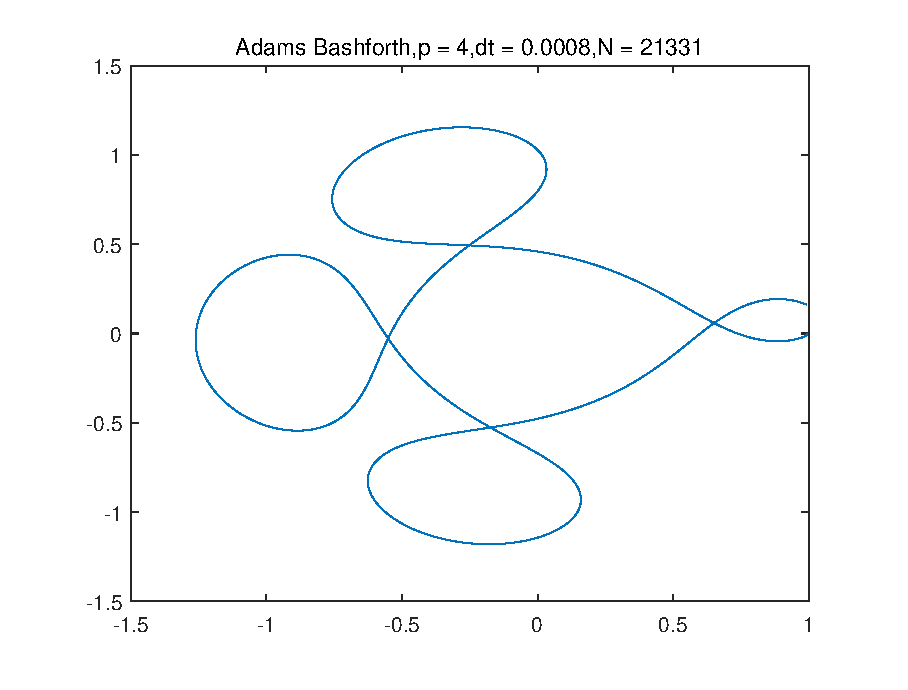
\includegraphics[width=1.5in]{Pictures/3_14.eps}}
	\caption{Adams-Bashforth,p = 3,4 }
	\label{AB2ks}
\end{figure}
\begin{table}[!htp]
	\centering
	\begin{tabular}{|c|c|}
		\hline	
		Order & Key time-step size  \\
		\hline		
		1 & $1\times 10^{-5}$ \\	
		\hline		
		2 & $1\times 10^{-4}$   \\	
		\hline 
		3 & $4\times 10^{-4}$  \\
		\hline
		4 & $8\times 10^{-4}$  \\
		\hline
	\end{tabular}
	\caption{Key time-step of Adams-Bashforth, Initial1}
	\label{tab:test31}
\end{table}
\begin{figure}[!htp] 
	\centering
	\subfigure[p = 2, dt = 4e-04]{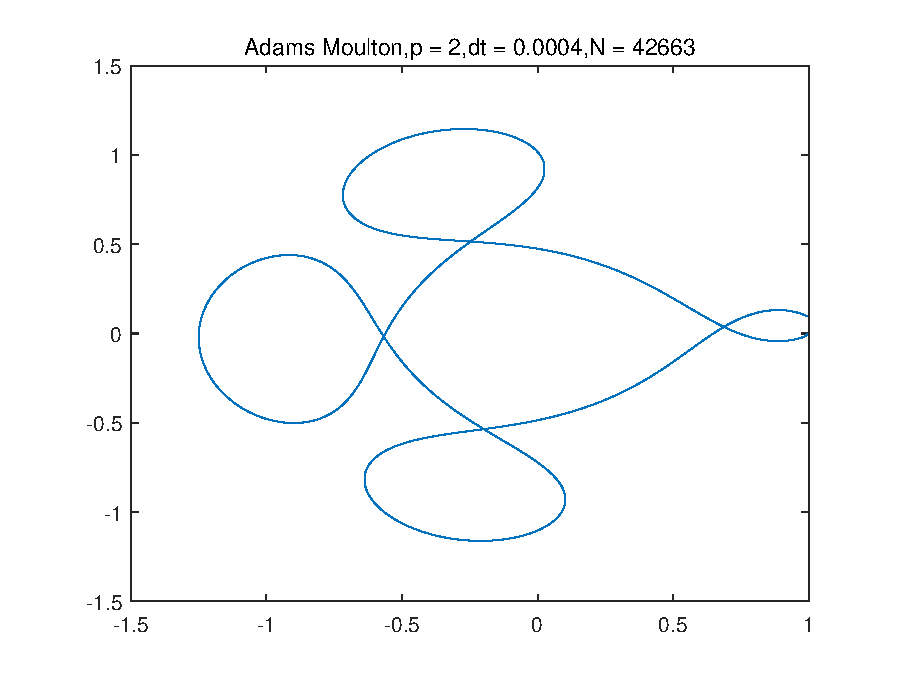
\includegraphics[width=1.5in]{Pictures/3_21.eps}}
	\subfigure[p = 3, dt = 0.001]{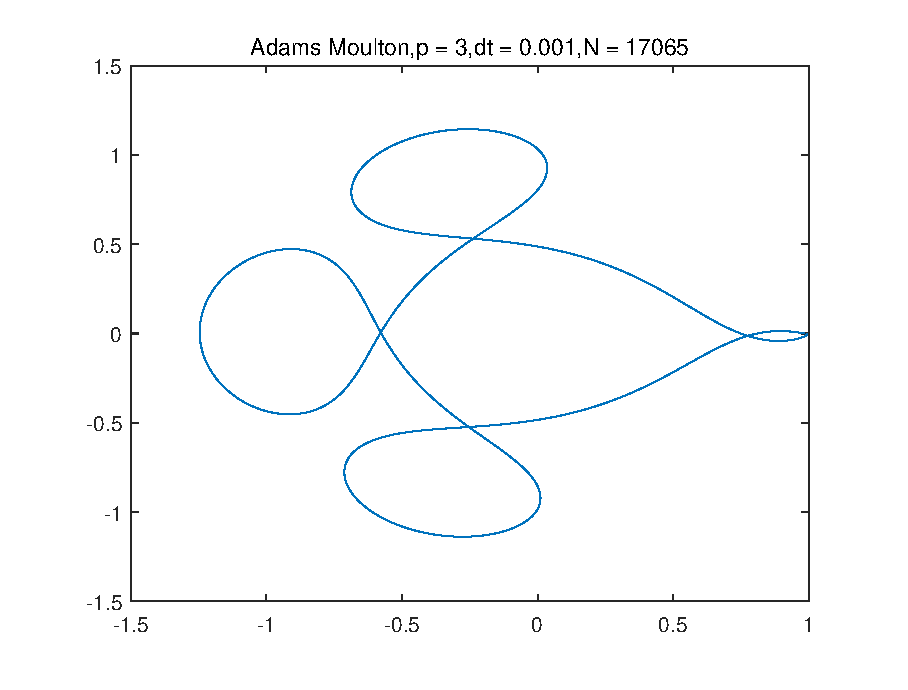
\includegraphics[width=1.5in]{Pictures/3_22.eps}}
	\caption{Adams-Moulton,p = 2,3 }
	\label{AM1ks}
\end{figure}
\begin{figure}[!htp] 
	\centering
	\subfigure[p = 4, dt = 0.002]{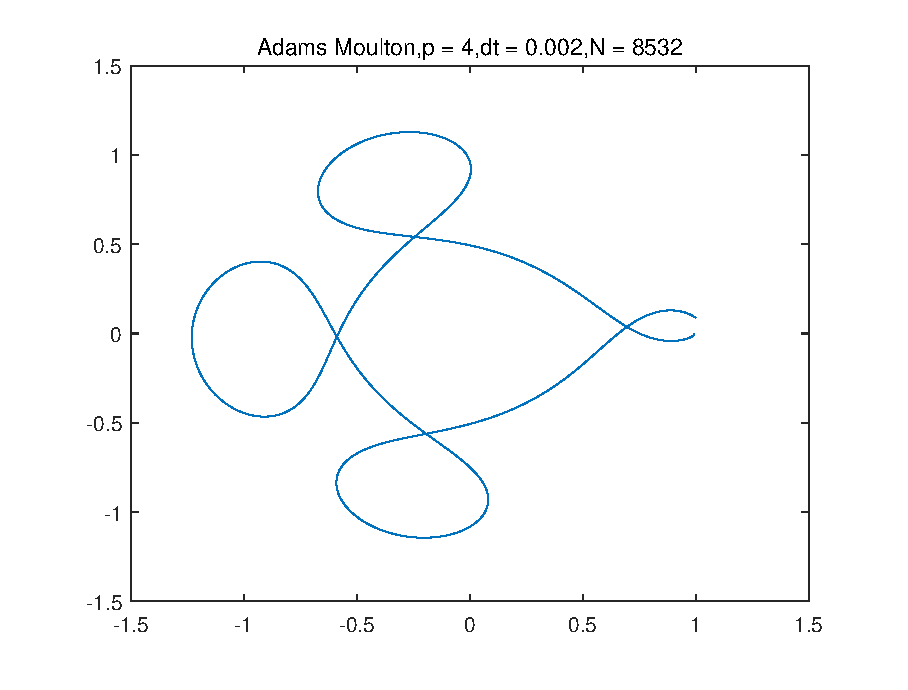
\includegraphics[width=1.5in]{Pictures/3_23.eps}}
	\subfigure[p = 5, dt = 0.001]{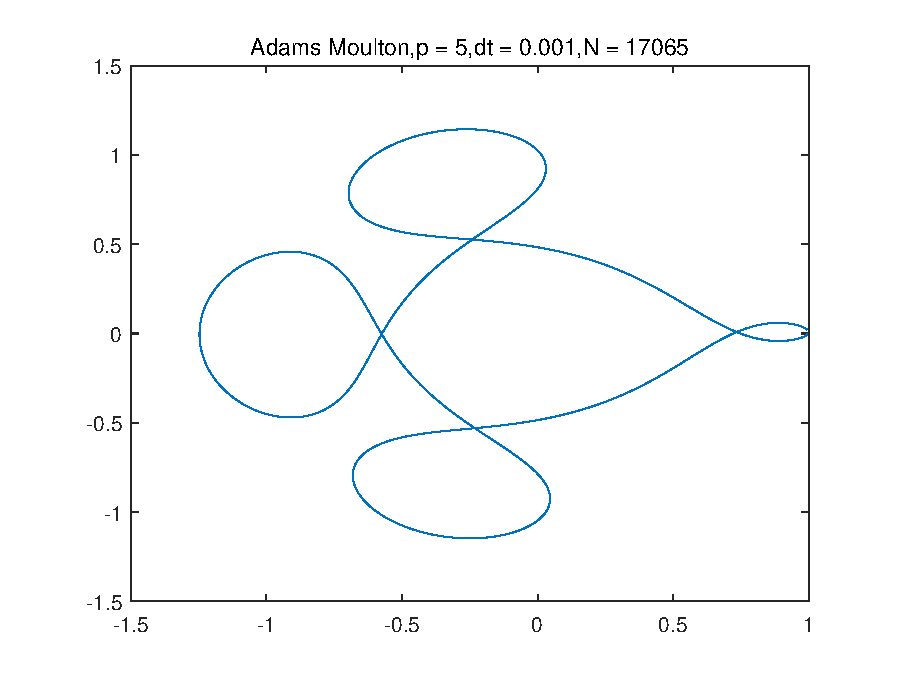
\includegraphics[width=1.5in]{Pictures/3_24.eps}}
	\caption{Adams-Moulton,p = 4,5 }
	\label{AM2ks}
\end{figure}

\begin{table}[!htp]
	\centering
	\begin{tabular}{|c|c|}
		\hline	
		Order & Key time-step size  \\
		\hline		
		2 & $4\times 10^{-4}$ \\	
		\hline		
		3 & $1\times 10^{-3}$   \\	
		\hline 
		4 & $2\times 10^{-3}$  \\
		\hline
		5 & $1\times 10^{-3}$  \\
		\hline
	\end{tabular}
	\caption{Key time-step of Adams-Moulton, Initial1}
	\label{tab:test32}
\end{table}
\begin{figure}[!htp] 
	\centering
	\subfigure[p = 1, dt = 1e-05]{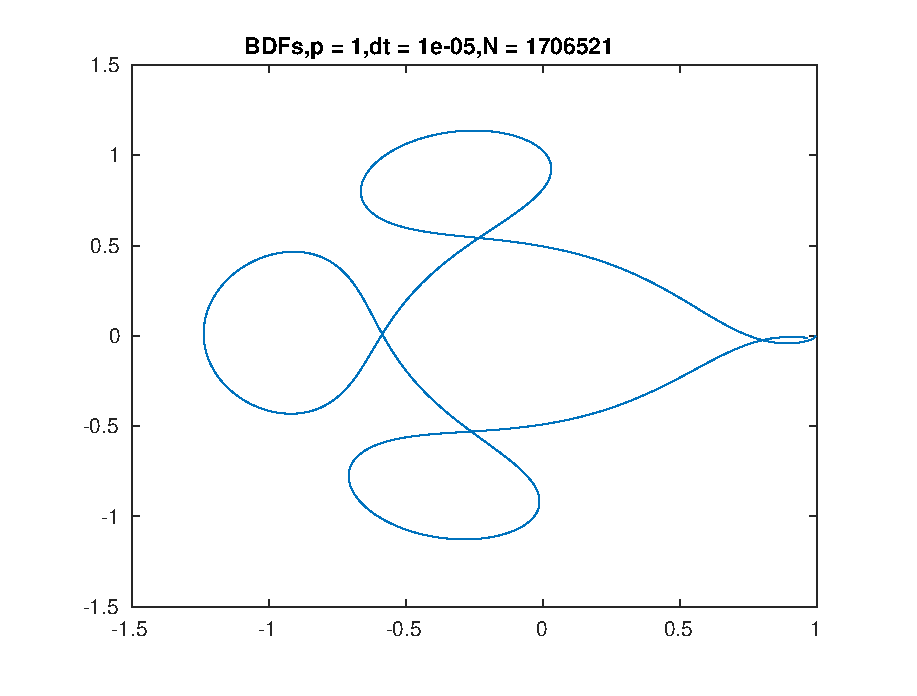
\includegraphics[width=1.5in]{Pictures/3_31.eps}}
	\subfigure[p = 2, dt = 1e-04]{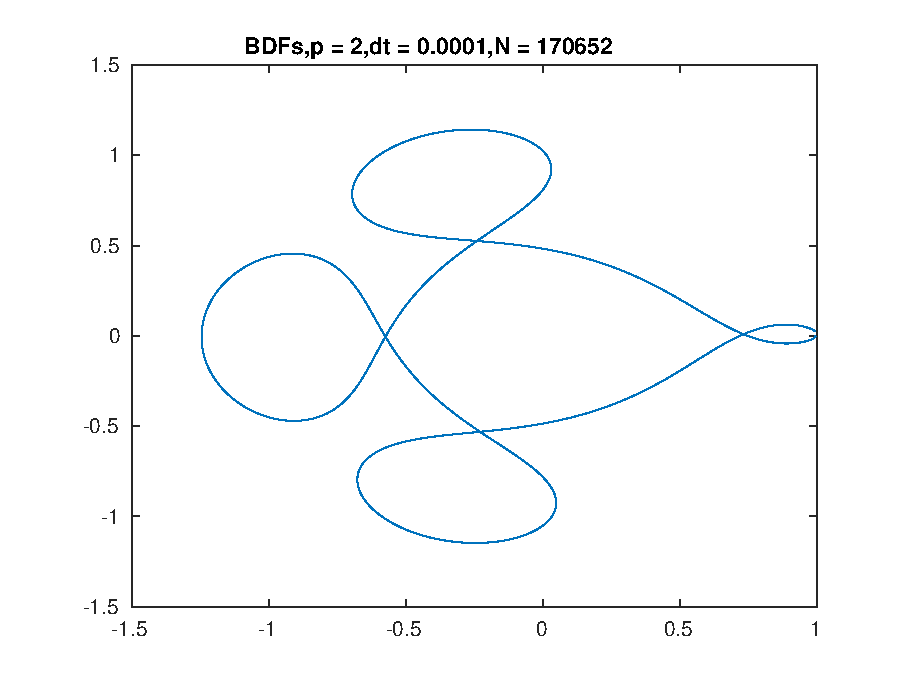
\includegraphics[width=1.5in]{Pictures/3_32.eps}}
	\caption{BDF,p = 1,2 }
	\label{BDF1ks}
\end{figure}
\begin{figure}[!htp] 
	\centering
	\subfigure[p = 3, dt = 4e-04]{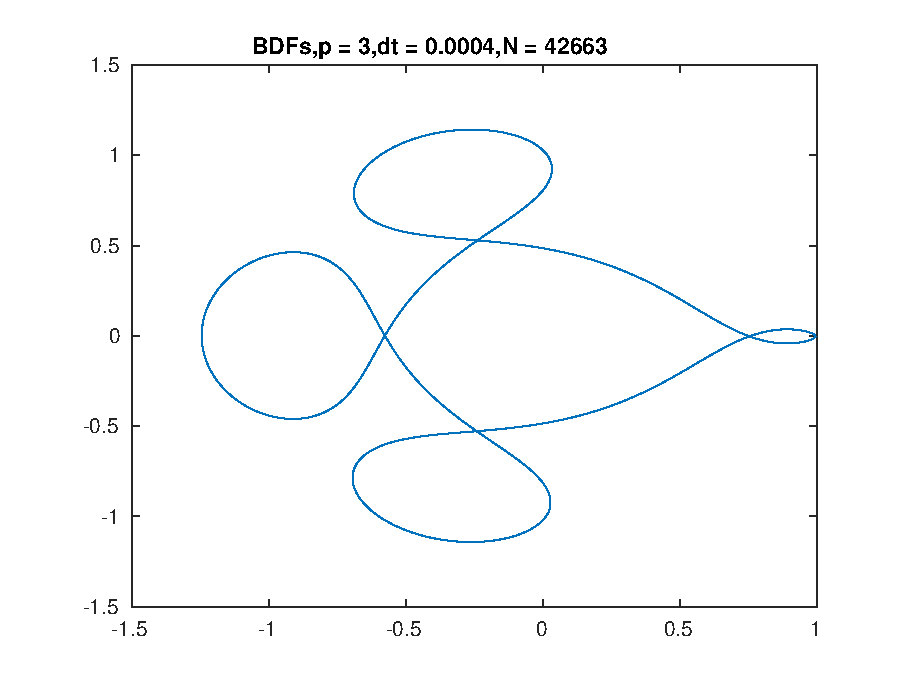
\includegraphics[width=1.5in]{Pictures/3_33.eps}}
	\subfigure[p = 4, dt = 0.001]{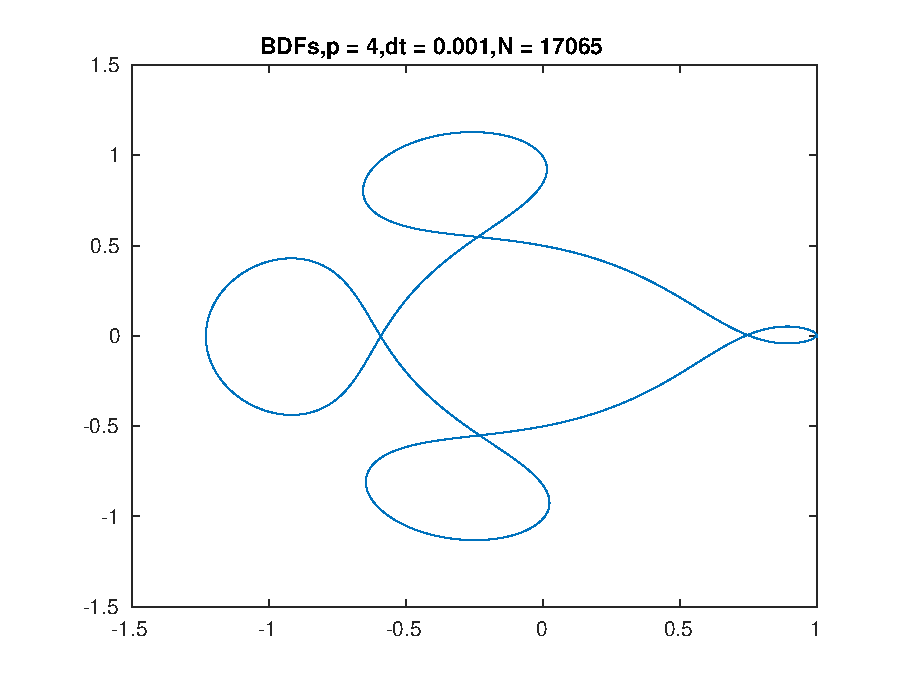
\includegraphics[width=1.5in]{Pictures/3_34.eps}}
	\caption{BDF,p = 3,4 }
	\label{BDF2ks}
\end{figure}
\begin{table}[!htp]
	\centering
	\begin{tabular}{|c|c|}
		\hline	
		Order & Key time-step size  \\
		\hline		
		1 & $1\times 10^{-5}$ \\	
		\hline		
		2 & $1\times 10^{-4}$   \\	
		\hline 
		3 & $4\times 10^{-4}$  \\
		\hline
		4 & $1\times 10^{-3}$  \\
		\hline
	\end{tabular}
	\caption{Key time-step of BDF, Initial1}
	\label{tab:test33}
\end{table}
\begin{figure}[!htp]   
	\centering
	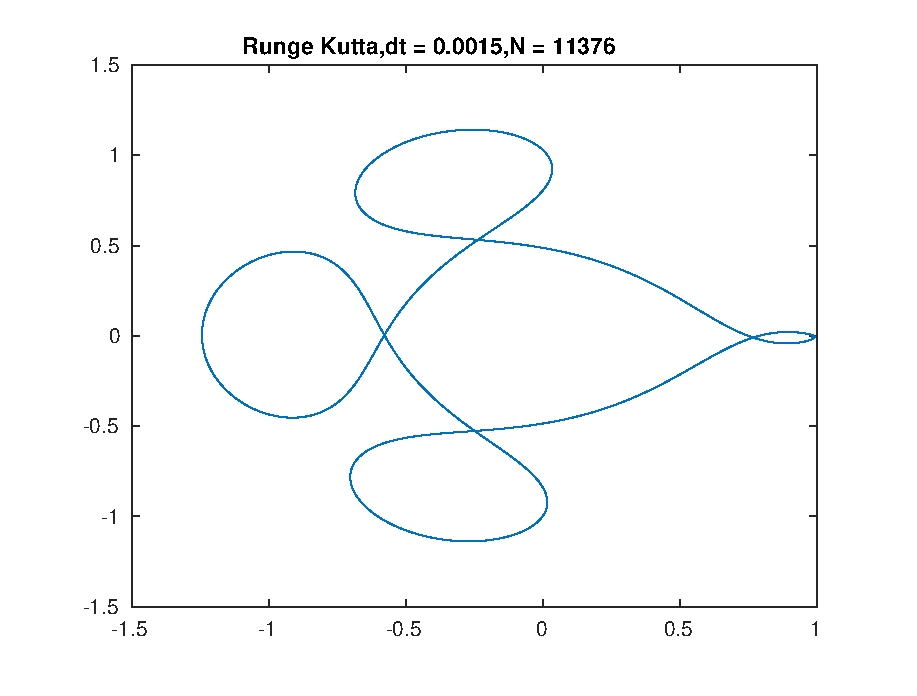
\includegraphics[width=6cm]{Pictures/3_4.eps}
	\caption{Runge-Kutta, dt = 0.0015, Initial1}
	\label{fig:RKks}
\end{figure}
\begin{table}[!htp]
	\centering
	\begin{tabular}{|c|c|}
		\hline	
		Order & Key time-step size  \\
		\hline		
		4 & $1.5\times 10^{-3}$ \\	
		\hline		
	\end{tabular}
	\caption{Key time-step of Runge-Kutta, Initial1}
	\label{tab:test34}
\end{table}
\newpage
\subsubsection{Time-step size for Initial2}
Similarly, reference plot of solution for Initial2 is as follows:
\begin{figure}[!htp]   
	\centering
	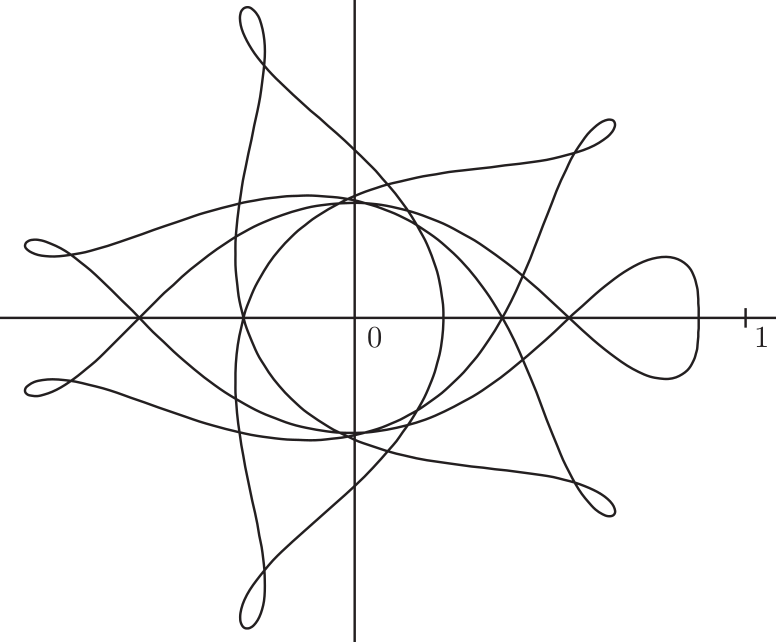
\includegraphics[width=6cm]{Pictures/I2.png}
	\caption{Reference plot for Initial2}
	\label{fig:R2}
\end{figure}\\
To avoid meaningless display of plots, we omit all figures and list all results in form of table. You can use the command \textbf{"make test32"} to get all the .m file, and run them to get corresponding plot.
\newpage
\begin{table}[!htp]
	\centering
	\begin{tabular}{|c|c|c|}
		\hline
		Method & Order & Key time-step size \\
		\hline	
		\multirow{4}{*}{Adams-Bashforth} & 1 & $1\times 10^{-5}$  \\
		\cline{2-3}		
		 & 2 &$5\times 10^{-3}$\\	
		\cline{2-3}		
		 & 3 &$5\times 10^{-3}$  \\	
		\cline{2-3} 
		 & 4 &$0.01$  \\
		\hline
		\multirow{4}{*}{Adams-Moulton} & 2 & $0.01$  \\
		\cline{2-3}		
		& 3 &$0.01$\\	
		\cline{2-3}		
		& 4 &$0.025$  \\	
		\cline{2-3} 
		& 5 &$0.025$  \\
		\hline
		\multirow{4}{*}{BDF} & 1 & $1\times 10^{-5}$  \\
		\cline{2-3}		
		& 2 &$5\times 10^{-3}$\\	
		\cline{2-3}		
		& 3 &$5\times 10^{-3}$  \\	
		\cline{2-3} 
		& 4 &$0.01$  \\
		\hline
		Runge-Kutta & 4 & $0.04$ \\
		\hline
	\end{tabular}
	\caption{Key time-step, Initial2}
	\label{tab:test35}
\end{table}
%4.Winner 每种方法取最快的 make test4
\subsection{Efficiency comparison of methods}
In the last part, we discuss the efficiency of different methods. Specifically, we will compare the running time when achieving an error of $10^{-3}$ based on the max-norm of the solution error. Since we are comparing relative efficiency, initial consition has little impact on the comparison.We take Initial1 as initial condition in the comparison below.\\
We take Euler's method as an example. The input file is as follows:
\begin{table}[!htp]
	\centering
	\begin{tabular}{|c|c|c|c|}
		\hline	
		Index & Method & Order & dt \\
		\hline		
		1 & Adams-Bashforth & 1 & 0.00000013   \\	
		\hline \hline
		Initial & N & err & grid-refine \\
		\hline
		Initial1 & 0 & 1 & 0 \\
		\hline
	\end{tabular}
	\caption{Input of Euler's method }
	\label{tab:4}
\end{table}\\
Run the program multiple times, we get:\\\\
\emph{err: 0.00100116,CPU time: 356232(ms)}\\
\emph{err: 0.00100116,CPU time: 358821(ms)}\\
\emph{err: 0.00100116,CPU time: 352904(ms)}\\
\emph{$\dots\dots$ }\\
\newpage
\noindent Take the average of CPU time as the final result, then the time we need to achieve required error for Euler's method is 428668 ms.\\
Similarly, for each method, We list results as follows. You can use the command \textbf{"make test4"} to get all the result\textbf{(will take much time)}. 
\begin{table}[!htp]
	\centering
	\begin{tabular}{|c|c|c|c|c|}
		\hline
		Method & Order & dt & err & CPU time(ms) \\
		\hline	
		\multirow{4}{*}{Adams-Bashforth} & 1 & $1.3\times 10^{-7}$ & $1.00\times 10^{-3}$ 
		& 356672\\
		\cline{2-5}		
		& 2 &$1.6\times 10^{-5}$&$ 1.00\times 10^{-3}$ & 4761.38\\	
		\cline{2-5}		
		& 3 &$1.3\times 10^{-4}$&$ 9.98\times 10^{-4}$ & 807.093 \\	
		\cline{2-5} 
		& 4 &$1.53\times 10^{-4}$&$ 9.98\times 10^{-4}$ & 855.834 \\
		\hline
		\multirow{4}{*}{Adams-Moulton} & 2 & $3.5\times 10^{-5}$&$ 9.51\times 10^{-4}$ 
		&  89518.2 \\
		\cline{2-5}		
		& 3 &$3.1\times 10^{-4}$& $ 9.91\times 10^{-4}$& 10260.8\\	
		\cline{2-5}		
		& 4 &$3\times 10^{-4}$ &$ 1.03\times 10^{-3}$& 10817.4\\	
		\cline{2-5} 
		& 5 &$4.6\times 10^{-4}$ &$ 1.02\times 10^{-3}$ & 7049.67\\
		\hline
		\multirow{4}{*}{BDF} & 1 & $< 1\times 10^{-6}$&$1.00\times 10^{-3}$ 
		& $>2\times 10^{7}$  \\
		\cline{2-5}		
		& 2 &$1.8\times 10^{-5}$& $ 1.00\times 10^{-3}$& 143806\\	
		\cline{2-5}		
		& 3 &$1.8\times 10^{-4}$ &$ 1.00\times 10^{-3}$ & 17498.1\\	
		\cline{2-5} 
		& 4 &$1.8\times 10^{-4}$ &$ 1.02\times 10^{-3}$ & 17652.3\\
		\hline
		Runge-Kutta & 4 & $6.9\times 10^{-4}$ &$ 1.02\times 10^{-3}$ & 265.41\\
		\hline
	\end{tabular}
	\caption{comparison of methods}
	\label{tab:test4}
\end{table}\\
Obviously the winner is the \textbf{classical Runge-Kutta method} in terms of total CPU time
to achieve an error of $10^{-3}$ of the solution error.
\end{document}
